\begin{name}
	{\tenchude}{\tendethi}{LỚP TOÁN THẦY PHÁT}{\thoigian}
\end{name}
\setcounter{ex}{0}\setcounter{bt}{0}
\Opensolutionfile{ans}[ans/ans-2-TT-18-TranHungDao-NamDinh-L1-23]
\begin{ex}%[Thi thử tốt nghiệp - THPT Trần Hưng Đạo - Nam Định - L1 - 2023]%[Lê Nguyễn Viết Tường - 12-EX-6-2032]%[2D4Y1-2]
Trên mặt phẳng tọa độ, điểm $M(-4;5)$ là điểm biểu diễn của số phức nào dưới đây?
\choice 
{\True $z=-4+5i$} 
{$z=-4-5i$}
{$z=4-5i$} 
{$z=-5+4i$}
\loigiai
{
$M(-4;5)$ là điểm biểu diễn của số phức $z=-4+5i$.
}
\end{ex}

\begin{ex}%[Thi thử tốt nghiệp - THPT Trần Hưng Đạo - Nam Định - L1 - 2023]%[Lê Nguyễn Viết Tường - 12-EX-6-2032]%[2H1Y3-2]
Cho hình chóp $S.ABC$ có đáy là tam giác đều cạnh $2a$, cạnh bên $SA$ vuông góc với đáy và $SA=a\sqrt{3}$. Tính thể tích $V$ của khối chóp $S.ABC$.
\choice 
{$V=\dfrac{3}{4}a^3$} 
{\True $V=a^3$}
{$V=2a^3\sqrt{2}$} 
{$V=\dfrac{1}{2}a^3$}
\loigiai
{
\immini{
Thể tích khối chóp $S.ABCD$ là
$$V=\dfrac{1}{3}SA\cdot S_{ABC}=\dfrac{1}{3}\cdot a\sqrt{3}\cdot\dfrac{(2a)^2\sqrt{3}}{4}=a^3.$$
}{
\begin{tikzpicture}[line cap=round,line join=round,scale=.7,>=stealth,font=\footnotesize ]
\tkzDefPoints{0/0/A,3/-2/B,5/0/C,0/4.5/S}
\tkzDrawSegments[dashed](A,C)
\tkzDrawSegments[](S,A S,B S,C A,B B,C)
\tkzLabelPoints[above](S)
\tkzLabelPoints[left](A)
\tkzLabelPoints[below](B)
\tkzLabelPoints[right](C)
\end{tikzpicture}
}
}
\end{ex}

\begin{ex}%[Thi thử tốt nghiệp - THPT Trần Hưng Đạo - Nam Định - L1 - 2023]%[Lê Nguyễn Viết Tường - 12-EX-6-2032]%[2D1Y1-1]
Cho hàm số $y=\dfrac{-x+2}{x-1}$. Khẳng định nào sau đây là khẳng định đúng?
\choice 
{Hàm số nghịch biến trên $(-\infty ;1)\cup (1;+\infty )$} 
{\True Hàm số nghịch biến trên mỗi khoảng $(-\infty ;1)$ và $(1;+\infty )$}
{Hàm số nghịch biến trên $\mathbb{R}$} 
{Hàm số đồng biến trên mỗi khoảng $(-\infty ;1)$ và $(1;+\infty )$}
\loigiai
{
Tập xác định: $\mathscr D=\mathbb{R}\setminus\{1\}$.\\
Ta có $y'=\dfrac{-1}{(x-1)^2}<0\,\,\,\forall x\in\mathscr D\Rightarrow y$ nghịch biến trên $(-\infty ;1)$ và $(1;+\infty )$.
}
\end{ex}

\begin{ex}%[Thi thử tốt nghiệp - THPT Trần Hưng Đạo - Nam Định - L1 - 2023]%[Lê Nguyễn Viết Tường - 12-EX-6-2032]%[2H3Y2-2]
Trong KG $Oxyz$, cho mặt phẳng $(P)\colon 2x-z+3=0$. Véc-tơ nào dưới đây là một véc-tơ pháp tuyến của mặt phẳng $(P)$?
\choice 
{\True $\overrightarrow{n}=(2;0;-1)$} 
{$\overrightarrow{n}=(2;0;3)$}
{$\overrightarrow{n}=(0;2;-1)$} 
{$\overrightarrow{n}=(2;-1;3)$}
\loigiai
{
$\overrightarrow{n}=(2;0;-1)$ là một véc-tơ pháp tuyến của mặt phẳng $(P)$.
}
\end{ex}

\begin{ex}%[Thi thử tốt nghiệp - THPT Trần Hưng Đạo - Nam Định - L1 - 2023]%[Lê Nguyễn Viết Tường - 12-EX-6-2032]%[2D2Y6-2]
Tập nghiệm của bất phương trình $5^{2x+3}>\dfrac{1}{25}$ là
\choice 
{\True $\left (-\dfrac{5}{2};+\infty  \right )$} 
{$\left (-\dfrac{1}{2};+\infty  \right )$}
{$(0;+\infty )$} 
{$\left (-\infty ;-\dfrac{5}{2} \right )$}
\loigiai
{
$$5^{2x+3}>\dfrac{1}{25}\Leftrightarrow 5^{2x+3}>5^{-2}\Leftrightarrow 2x+3>-2\Leftrightarrow x>-\dfrac{5}{2}.$$
Phương trình đã cho có tập nghiệm $S=\left (-\dfrac{5}{2};+\infty  \right )$.
}
\end{ex}

\begin{ex}%[Thi thử tốt nghiệp - THPT Trần Hưng Đạo - Nam Định - L1 - 2023]%[Lê Nguyễn Viết Tường - 12-EX-6-2032]%[1H3Y3-2]
Cho hình chóp $S.ABC$ có $SA$ vuông góc với $(ABC)$, tam giác $ABC$ đều cạnh bằng $a$, $SA=a\sqrt{3}$. Góc giữa đường thẳng $SC$ và mặt phẳng $(ABC)$ bằng
\choice 
{$90^{\circ}$} 
{\True $60^{\circ}$}
{$30^{\circ}$} 
{$45^{\circ}$}
\loigiai
{
\immini{
$SA\perp (ABC)\Rightarrow AC$ là hình chiếu vuông góc của $SC$ lên $(ABC)$\\$\Rightarrow\widehat{SCA}$ là góc giữa $SC$ và mặt phẳng $(ABC)$.\\
$\triangle SAC$ vuông tại $A\Rightarrow\tan\widehat{SCA}=\dfrac{SA}{AC}=\sqrt{3}\Rightarrow\widehat{SCA}=60^{\circ}$.\\
Vậy góc giữa $SC$ và mặt phẳng $(ABC)$ bằng $60^{\circ}$.
}{
\begin{tikzpicture}[line cap=round,line join=round,scale=.7,>=stealth,font=\footnotesize ]
\tkzDefPoints{0/0/A,3/-2/B,5/0/C,0/4.5/S}
\tkzDrawSegments[dashed](A,C)
\tkzDrawSegments[](S,A S,B S,C A,B B,C)
\tkzLabelPoints[above](S)
\tkzLabelPoints[left](A)
\tkzLabelPoints[below](B)
\tkzLabelPoints[right](C)
\end{tikzpicture}
}
}
\end{ex}

\begin{ex}%[Thi thử tốt nghiệp - THPT Trần Hưng Đạo - Nam Định - L1 - 2023]%[Lê Nguyễn Viết Tường - 12-EX-6-2032]%[2H3Y2-5]
Trong không gian với hệ trục tọa độ $Oxyz$, góc giữa hai mặt phẳng $(Oxy)$ và $(Oxz)$ bằng
\choice 
{$45^{\circ}$} 
{$30^{\circ}$}
{\True $90^{\circ}$} 
{$60^{\circ}$}
\loigiai
{
Trong KG $Oxyz$, các mặt phẳng $(Oxy)$, $(Oyz)$ và $(Oxz)$ đôi một vuông góc với nhau. Do đó góc giữa hai mặt phẳng $(Oxy)$ và $(Oxz)$ bằng $90^{\circ}$.
}
\end{ex}

\begin{ex}%[Thi thử tốt nghiệp - THPT Trần Hưng Đạo - Nam Định - L1 - 2023]%[Lê Nguyễn Viết Tường - 12-EX-6-2032]%[2H3Y3-2]
Trong KG $Oxyz$, cho đường thẳng $d\colon \dfrac{x-1}{2}=\dfrac{y+3}{-1}=\dfrac{z}{3}$. PTTS của đường thẳng $d$ là
\choice 
{$\heva{& x=2+t\\&y=-1-3t\\&z=3 }$} 
{$\heva{& x=1+2t\\&y=3-t\\&z=3t }$}
{\True $\heva{& x=1+2t\\&y=-3-t\\&z=3t }$} 
{$\heva{& x=-2+t\\&y=1-3t \\z=3}$}
\loigiai
{
$d$ đi qua $A(1;-3;0)$ có một véc-tơ chỉ phương $\overrightarrow{u}=(2;-1;3)\Rightarrow d\colon\heva{& x=1+2t\\&y=-3-t\\&z=3t }$.
}
\end{ex}

\begin{ex}%[Thi thử tốt nghiệp - THPT Trần Hưng Đạo - Nam Định - L1 - 2023]%[Lê Nguyễn Viết Tường - 12-EX-6-2032]%[2H3Y1-3]
Trong KG $Oxyz$ cho mặt cầu $(S)$ có phương trình $x^2+y^2+z^2-2x+4y-6z-2=0$. Đường kính của mặt cầu $(S)$ là
\choice 
{$\sqrt{14}$} 
{$4$}
{$2\sqrt{14}$} 
{\True $8$}
\loigiai
{
$(S)$ có tâm $I(1;-2;3)$ bán kính $R=\sqrt{1^2+(-2)^2+3^2-(-2)}=4$.\\
Khi đó đường kính của $(S)$ là $2\cdot 4=8$.
}
\end{ex}

\begin{ex}%[Thi thử tốt nghiệp - THPT Trần Hưng Đạo - Nam Định - L1 - 2023]%[Lê Nguyễn Viết Tường - 12-EX-6-2032]%[2D1Y5-4]
Đồ thị hàm số $y=\dfrac{x+2022}{x+2023}$ cắt trục hoành tại điểm có tọa độ là
\choice 
{$(0;-2023)$} 
{\True $(-2022;0)$}
{$(2023;0)$} 
{$(0;2023)$}
\loigiai
{
Thay $y=0$ vào $y=\dfrac{x+2022}{x+2023}$ ta được $x=-2022$.\\
Do đó đồ thị hàm số đã cho cắt trục hoành tại điểm có tọa độ là $(-2022;0)$.
}
\end{ex}

\begin{ex}%[Thi thử tốt nghiệp - THPT Trần Hưng Đạo - Nam Định - L1 - 2023]%[Lê Nguyễn Viết Tường - 12-EX-6-2032]%[2D2Y6-1]
Tìm tập nghiệm của bất phương trình $\log_{\tfrac{1}{3}}(x-3)<-2$.
\choice 
{\True $(12;+\infty )$} 
{$(-\infty ;12)$}
{$\left (-\infty ;\dfrac{7}{3} \right )$} 
{$(3;12)$}
\loigiai
{
Điệu kiện: $x>3$.\\
Ta có
$$\log_{\tfrac{1}{3}}(x-3)<-2\Leftrightarrow x-3>\left (\dfrac{1}{3} \right )^{-2}\Leftrightarrow x-3>9\Leftrightarrow x>12.$$
So sánh điều kiện ta được tập nghiệm của bất phương trình đã cho là $(12;+\infty )$.
}
\end{ex}

\begin{ex}%[Thi thử tốt nghiệp - THPT Trần Hưng Đạo - Nam Định - L1 - 2023]%[Lê Nguyễn Viết Tường - 12-EX-6-2032]%[2D4Y1-1]
Mô-đun của số phức $z=3+4i$ bằng
\choice 
{$\sqrt{5}$} 
{\True $5$}
{$25$} 
{$7$}
\loigiai
{
Ta có $|z|=\sqrt{3^2+4^2}=5$.
}
\end{ex}

\begin{ex}%[Thi thử tốt nghiệp - THPT Trần Hưng Đạo - Nam Định - L1 - 2023]%[Lê Nguyễn Viết Tường - 12-EX-6-2032]%[1D2Y2-1]
Cho tập hợp $A$ có $10$ phần tử, số tập con gồm $2$ phần tử của $A$ là
\choice 
{$\mathrm{A}_{10}^2$} 
{$10^2$}
{\True $\mathrm{C}_{10}^2$} 
{$\mathrm{A}_{10}^8$}
\loigiai
{
Số tập con gồm $2$ phần tử của $A$ là $\mathrm{C}_{10}^2$.
}
\end{ex}

\begin{ex}%[Thi thử tốt nghiệp - THPT Trần Hưng Đạo - Nam Định - L1 - 2023]%[Lê Nguyễn Viết Tường - 12-EX-6-2032]%[2D1Y1-2]
\immini{
Cho hàm số $y=f(x)=ax^3+bx^2+cx+d$ có đồ thị như hình vẽ bên. Hàm số $y=f(x)$ đồng biến trên khoảng nào dưới đây?
\choice 
{$(-1;1)$} 
{$(-\infty ;-1)$}
{$(2;+\infty )$} 
{\True $(0;1)$}
}{
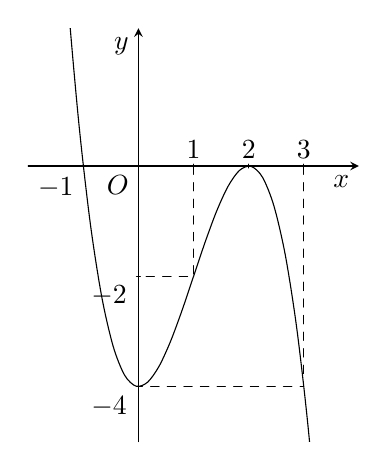
\begin{tikzpicture}[line cap=round,line join=round,scale=.7,>=stealth]
\draw[->] (-2,0)--(4,0) node[below left] {$x$};
\draw[->] (0,-5)--(0,2.5) node[below left] {$y$};
\draw (0,0) node [below left] {$O$};
\foreach \x in {1,2,3}
\draw[thin] (\x,1pt)--(\x,-1pt) node[above] {$\x$};
\draw[thin] (-1,1pt)--(-1,-1pt) node[below left] {$-1$};
\foreach \y in {-2,-4}
\draw[thin] (1pt,\y)--(-1pt,\y) node[below left] {$\y$};
\begin{scope}
\clip (-2,-5) rectangle (4,2.5);
\draw[domain=-1.5:3.5,smooth,variable=\x] plot (\x,{-(\x)^3+3*(\x)^2-4});
\end{scope}
\draw[dashed,thin](3,0)--(3,-4)--(0,-4);
\draw[dashed,thin](1,0)--(1,-2)--(0,-2);

\end{tikzpicture}
}
\loigiai
{
Dựa vào đồ thị hàm số ta thấy $y=f(x)$ đồng biến trên $(0;2)$.\\
Mà $(0;1)\subset (0;2)$. Nên hàm số đã cho đồng biến trên $(0;1)$.
}
\end{ex}

\begin{ex}%[Thi thử tốt nghiệp - THPT Trần Hưng Đạo - Nam Định - L1 - 2023]%[Lê Nguyễn Viết Tường - 12-EX-6-2032]%[2D2Y4-1]
Tập xác định của hàm số $y=(\pi +1)^x$ là
\choice 
{$\mathbb{R}\setminus \{0\}$} 
{$(-1;+\infty )$}
{$(0;+\infty )$} 
{\True $\mathbb{R}$}
\loigiai
{
Ta có $\pi +1>0$. Do đó hàm số đã cho có tập xác định là $\mathbb{R}$.
}
\end{ex}

\begin{ex}%[Thi thử tốt nghiệp - THPT Trần Hưng Đạo - Nam Định - L1 - 2023]%[Lê Nguyễn Viết Tường - 12-EX-6-2032]%[2D1Y4-1]
Đường thẳng nào dưới đây là đường tiệm cận ngang của đồ thị hàm số $y=\dfrac{x-3}{2x+1}$?
\choice 
{$x=-\dfrac{1}{2}$} 
{\True $y=\dfrac{1}{2}$}
{$y=-\dfrac{1}{2}$} 
{$x=\dfrac{1}{2}$}
\loigiai
{
Ta có $\lim\limits_{x\to +\infty }y=\lim\limits_{x\to +\infty }\dfrac{x-3}{2x+1}=\lim\limits_{x\to +\infty }\dfrac{1-\dfrac{3}{x}}{2+\dfrac{1}{x}}=\dfrac{1}{2}$.\\
Do đó $y=\dfrac{1}{2}$ là tiệm cận ngang của đồ thị hàm số đã cho.
}
\end{ex}

\begin{ex}%[Thi thử tốt nghiệp - THPT Trần Hưng Đạo - Nam Định - L1 - 2023]%[Lê Nguyễn Viết Tường - 12-EX-6-2032]%[2D1Y2-2]
Cho hàm số $f(x)$ có bảng biến thiên như sau
\begin{center}

\begin{tikzpicture}
\tkzTabInit[nocadre=false, lgt=1.2, espcl=2.2, deltacl=0.6]
{$x$/0.6, $f'(x)$/0.6, $f(x)$/2}
{$-\infty$,$0$,$3$,$+\infty$}
\tkzTabLine{,+,z,-,z,+,}
\tkzTabVar{-/$-\infty $,+/$2$,-/$-5$,+/$+\infty $}
\end{tikzpicture}
\end{center}
Điểm cực tiểu của hàm số đã cho là
\choice 
{$(0;2)$} 
{$y=-5$}
{\True $x=3$} 
{$(3;-5)$}
\loigiai
{
Dựa vào bảng biến thiên, điểm cực tiểu của hàm số đã cho là $x=3$.
}
\end{ex}

\begin{ex}%[Thi thử tốt nghiệp - THPT Trần Hưng Đạo - Nam Định - L1 - 2023]%[Lê Nguyễn Viết Tường - 12-EX-6-2032]%[2D2Y4-2]
Trên khoảng $(0;+\infty )$, đạo hàm của hàm số $y=\log_{2023}x$ là
\choice 
{$y'=\dfrac{1}{x}$} 
{$y'=\dfrac{\ln 2023}{x}$}
{\True $y'=\dfrac{1}{x\ln 2023}$} 
{$y'=\dfrac{-1}{x\ln 2023}$}
\loigiai
{
Ta có $\left (\log_{2023}x \right )'=\dfrac{1}{x\ln 2023}$.
}
\end{ex}

\begin{ex}%[Thi thử tốt nghiệp - THPT Trần Hưng Đạo - Nam Định - L1 - 2023]%[Lê Nguyễn Viết Tường - 12-EX-6-2032]%[2H2Y1-2]
Cho hình nón có bán kính đáy $r=3$ và độ dài đường sinh $l=6$. Diện tích xung quanh của hình nón đã cho bằng
\choice 
{$6\pi$} 
{$36\pi$}
{$108\pi$} 
{\True $18\pi$}
\loigiai
{
Diện tích xung quanh của hình nón là $$S_{\text{xq}}=\pi rl=18\pi.$$
}
\end{ex}

\begin{ex}%[Thi thử tốt nghiệp - THPT Trần Hưng Đạo - Nam Định - L1 - 2023]%[Lê Nguyễn Viết Tường - 12-EX-6-2032]%[2H3Y1-1]
Trong KG $Oxyz$, cho điểm $M(3;2;-1)$. Khi đó điểm đối xứng với $M$ qua mặt phẳng $(Oyz)$ có tọa độ bằng
\choice 
{$(3;-2;1)$} 
{$(3;0;0)$}
{\True $(-3;2;-1)$} 
{$(0;2;-1)$}
\loigiai
{
Điểm đối xứng với $M$ qua mặt phẳng $(Oyz)$ có tọa độ bằng $(-3;2;-1)$.
}
\end{ex}

\begin{ex}%[Thi thử tốt nghiệp - THPT Trần Hưng Đạo - Nam Định - L1 - 2023]%[Lê Nguyễn Viết Tường - 12-EX-6-2032]%[2D2B3-2]
Cho $\log_{a}b=3,\log_{a}c=-4$. Khi đó $P=\log_{a}\left (\dfrac{a^3\sqrt{c}}{b^2} \right )$ bằng bao nhiêu?
\choice 
{$P=-5$} 
{$P=-1$}
{\True $P=7$} 
{$P=11$}
\loigiai
{
$$P=\log_{a}\left (\dfrac{a^3\sqrt{c}}{b^2} \right )=\log_{a}a^3+\log_{a}\sqrt{c}-\log_{a}b^2=3\log_{a}a+\dfrac{1}{2}\log_{a}c-2\log_{a}b=3+\dfrac{1}{2}\cdot (-4)+2\cdot 3=7.$$
}
\end{ex}

\begin{ex}%[Thi thử tốt nghiệp - THPT Trần Hưng Đạo - Nam Định - L1 - 2023]%[Lê Nguyễn Viết Tường - 12-EX-6-2032]%[1D3B3-2]
Cho cấp số cộng $\left (u_n \right )$, biết $u_5-u_1=20$. Tìm công sai $d$ của cấp số cộng.
\choice 
{\True $d=5$} 
{$d=4$}
{$d=-4$} 
{$d=-5$}
\loigiai
{
Ta có 
$$u_5-u_1=20\Leftrightarrow u_1+4d-u_1=20\Leftrightarrow d=5.$$
}
\end{ex}

\begin{ex}%[Thi thử tốt nghiệp - THPT Trần Hưng Đạo - Nam Định - L1 - 2023]%[Lê Nguyễn Viết Tường - 12-EX-6-2032]%[2D3B1-1]
Biết $\displaystyle\int f(x)\mathrm{\,d}x=\dfrac{5^x}{\ln 5}+3x+C$, khi đó $f(x)$ bằng
\choice 
{$f(x)=\dfrac{5^x}{\ln 5}+3$} 
{$f(x)=\dfrac{5^x}{\ln 5}+3x$}
{$f(x)=5^x+3x$} 
{\True $f(x)=5^x+3$}
\loigiai
{
Ta có $\left(\dfrac{5^x}{\ln 5}+3x+C\right)'=\dfrac{1}{\ln 5}\cdot 5^x\cdot\ln x+3=5^x+3$.\\
Do đó $f(x)=5^x+3$.
}
\end{ex}

\begin{ex}%[Thi thử tốt nghiệp - THPT Trần Hưng Đạo - Nam Định - L1 - 2023]%[Lê Nguyễn Viết Tường - 12-EX-6-2032]%[2D3B2-1]
Nếu $\displaystyle\int\limits_{-1}^{3}f(x)\mathrm{\,d}x=-5$ và $\displaystyle\int\limits_{3}^{5}f(x)\mathrm{\,d}x=1$ thì $\displaystyle\int\limits_{-1}^{5}f(x)\mathrm{\,d}x$ bằng
\choice 
{$4$} 
{$-6$}
{$6$} 
{\True $-4$}
\loigiai
{
$$\displaystyle\int\limits_{-1}^{5}f(x)\mathrm{\,d}x=\displaystyle\int\limits_{-1}^{3}f(x)\mathrm{\,d}x+\displaystyle\int\limits_{3}^{5}f(x)\mathrm{\,d}x=-5+1=-4.$$
}
\end{ex}

\begin{ex}%[Thi thử tốt nghiệp - THPT Trần Hưng Đạo - Nam Định - L1 - 2023]%[Lê Nguyễn Viết Tường - 12-EX-6-2032]%[2D4B2-2]
Tìm số phức liên hợp của số phức $z=i(3i+1)$.
\choice 
{$\overline{z}=-3+i$} 
{$\overline{z}=3+i$}
{$\overline{z}=3-i$} 
{\True $\overline{z}=-3-i$}
\loigiai
{
Ta có $z=3i^2+i=-3+i$.\\
Do đó $\overline{z}=-3-i$.
}
\end{ex}

\begin{ex}%[Thi thử tốt nghiệp - THPT Trần Hưng Đạo - Nam Định - L1 - 2023]%[Lê Nguyễn Viết Tường - 12-EX-6-2032]%[2D1B2-2]
Cho hàm số $f(x)$ có đạo hàm $f'(x)=(2x+1)(x+2)^2(3x-1)^4$ với mọi $x\in\mathbb{R}$. Số điểm cực trị của đồ thị hàm số $f(x)$ là
\choice 
{$3$} 
{\True $1$}
{$2$} 
{$0$}
\loigiai
{
$f'(x)=0\Leftrightarrow \hoac{& x=-2\\&x=-\dfrac{1}{2}\\&x=\dfrac{1}{3} .}$\\
Bảng xét dấu
\begin{center}

\begin{tikzpicture}
\tkzTabInit[nocadre=false, lgt=1.2, espcl=2.2, deltacl=0.6]
{$x$/1, $f'(x)$/0.6}
{$-\infty$,$-2$,$-\dfrac{1}{2}$,$\dfrac{1}{3}$,$+\infty$}
\tkzTabLine{,-,z,-,z,+,z,+,}
\end{tikzpicture}
\end{center}
Ta thấy $f'(x)$ đổi dấu 1 lần. Do đó đồ thị hàm số đã cho có $1$ điểm cực trị.
}
\end{ex}

\begin{ex}%[Thi thử tốt nghiệp - THPT Trần Hưng Đạo - Nam Định - L1 - 2023]%[Lê Nguyễn Viết Tường - 12-EX-6-2032]%[2D3B2-1]
Nếu $\displaystyle\int\limits_{0}^{6}f(x)\mathrm{\,d}x=3$ thì $\displaystyle\int\limits_{0}^{6}\left [x+f(x) \right ]\mathrm{\,d}x$ bằng
\choice 
{$9$} 
{$39$}
{\True $21$} 
{$6$}
\loigiai
{
$$\displaystyle\int\limits_{0}^{6}\left [x+f(x) \right ]\mathrm{\,d}x=\displaystyle\int\limits_{0}^{6}x\mathrm{\,d}x+\displaystyle\int\limits_{0}^{6}f(x)\mathrm{\,d}x=\dfrac{x^2}{2}\,\Big |_{0}^{6}+3=21.$$
}
\end{ex}

\begin{ex}%[Thi thử tốt nghiệp - THPT Trần Hưng Đạo - Nam Định - L1 - 2023]%[Lê Nguyễn Viết Tường - 12-EX-6-2032]%[2D1B5-1]
\immini{
Hàm số nào dưới đây có đồ thị như hình vẽ?
\choice 
{$y=\dfrac{2x-2}{x-1}$} 
{$y=\dfrac{2x+1}{x-1}$}
{$y=\dfrac{x+2}{x+1}$} 
{\True $y=\dfrac{2x-1}{x+1}$}
}{
\begin{tikzpicture}[line cap=round,line join=round,scale=.7,>=stealth]
\draw[->] (-5,0)--(3,0) node[below left] {$x$};
\draw[->] (0,-2)--(0,6) node[below left] {$y$};
\draw (0,0) node [below left] {$O$};
\foreach \x in {-1}
\draw[thin] (\x,1pt)--(\x,-1pt) node[below left] {$\x$};
\foreach \y in {2}
\draw[thin] (1pt,\y)--(-1pt,\y) node[above right] {$\y$};
\begin{scope}
\clip (-5,-2) rectangle (3,6);
\draw[domain=-5:-1.2,smooth,variable=\x] plot (\x,{(2*(\x)-1)/((\x)+1)});
\draw[domain=-.8:3,smooth,variable=\x] plot (\x,{(2*(\x)-1)/((\x)+1)});
\end{scope}
\draw[dashed,thin](-5,2)--(3,2);
\draw[dashed,thin](-1,-2)--(-1,6);

\end{tikzpicture}
}
\loigiai
{
Đồ thị hàm số có tiệm cận đứng $x=-1$ do đó loại phương án $y=\dfrac{2x-2}{x-1}$ và $y=\dfrac{2x+1}{x-1}$.\\
Đồ thị hàm số có tiệm cận ngang $y=2$ do đó loại phương án $y=\dfrac{x+2}{x+1}$.\\
Vậy hàm số cần tìm là $y=\dfrac{2x-1}{x+1}$.
}
\end{ex}

\begin{ex}%[Thi thử tốt nghiệp - THPT Trần Hưng Đạo - Nam Định - L1 - 2023]%[Lê Nguyễn Viết Tường - 12-EX-6-2032]%[2H1B3-2]
Cho khối lăng trụ đứng có cạnh bên bằng $5$, đáy là hình vuông có cạnh bằng $4$. Thể tích khối lăng trụ bằng
\choice 
{$60$} 
{\True $80$}
{$100$} 
{$20$}
\loigiai
{
Chiều cao của hình lăng trụ là $h=5$.\\
Diện tích đáy hình lăng trụ là $S=4^2=16$.\\
Thể tích hình lăng trụ là $V=S\cdot h=16\cdot 5=80 $.
}
\end{ex}

\begin{ex}%[Thi thử tốt nghiệp - THPT Trần Hưng Đạo - Nam Định - L1 - 2023]%[Lê Nguyễn Viết Tường - 12-EX-6-2032]%[2H3B3-2]
Trong KG $Oxyz$, PTĐT đi qua $A(1;-2;0)$ và vuông góc với mặt phẳng $(P)\colon x-2y+2z+1=0$ là
\choice 
{$\dfrac{x-1}{1}=\dfrac{y-2}{-2}=\dfrac{z}{2}$} 
{$\dfrac{x-1}{1}=\dfrac{y-2}{1}=\dfrac{z}{-2}$}
{\True $\dfrac{x-1}{1}=\dfrac{y+2}{-2}=\dfrac{z}{2}$} 
{$\dfrac{x-1}{1}=\dfrac{y-2}{2}=\dfrac{z}{2}$}
\loigiai
{
$(P)$ có một véc-tơ pháp tuyến $\overrightarrow{n}=(1;-2;2)$.\\
Gọi $d$ là đường thẳng cần tìm.\\
Vì $d\perp (P)$ nên $\overrightarrow{n}$ là véc-tơ chỉ phương của $d$.\\
Khi đó $d\colon\dfrac{x-1}{1}=\dfrac{y+2}{-2}=\dfrac{z}{2}$.
}
\end{ex}

\begin{ex}%[Thi thử tốt nghiệp - THPT Trần Hưng Đạo - Nam Định - L1 - 2023]%[Lê Nguyễn Viết Tường - 12-EX-6-2032]%[2H3B3-7]
Cho mặt cầu $(S)$ tâm $O$, bán kính $R=3$. Một mặt phẳng $(P)$ cắt $(S)$ theo giao tuyến là đường tròn $(C)$ sao cho khoảng cách từ điểm $O$ đến mặt phẳng $(P)$ bằng $1$. Chu vi đường tròn $(C)$ bằng
\choice 
{\True $4\sqrt{2}\pi$} 
{$2\sqrt{2}\pi$}
{$8\pi$} 
{$4\pi$}
\loigiai
{
\immini{
Bán kính của đường tròn $(C)$ là $$r=\sqrt{R^2-\left [\mathrm{d}(O,(P) \right ]^2}=\sqrt{3^2-1^2}=2\sqrt{2}.$$
Chu vi của đường tròn $(C)$ là $$P=2\pi r=4\sqrt{2}\pi.$$
}{
\begin{tikzpicture}[line cap=round,line join=round,scale=1,>=stealth,font=\footnotesize ]
\tkzDefPoints{0/0/O,3/0/A,0/-1.7/I,1/-1.7/I1}
\tkzDrawCircle(O,A)
\tkzInterLC(I,I1)(O,A)\tkzGetFirstPoint{M}
\tkzDrawPoints[fill=black](O,I)
\draw[dashed](A) arc (0:180: 3 and .5);
\draw[](A) arc (0:-180: 3 and .5);
\draw[dashed](M) arc (0:180: 2.48 and .3);
\draw[](M) arc (0:-180: 2.48 and .3);
\tkzLabelPoints[left](O)
\tkzDrawSegments[dashed](O,I	I,M O,M)
\end{tikzpicture}
}
}
\end{ex}

\begin{ex}%[Thi thử tốt nghiệp - THPT Trần Hưng Đạo - Nam Định - L1 - 2023]%[Lê Nguyễn Viết Tường - 12-EX-6-2032]%[2D3B1-1]
Cho hàm số $f(x)$ thỏa mãn $f'(x)=4-3\sin x$ và $f(0)=5$. Tìm hàm số $f(x)$.
\choice 
{$f(x)=4x+3\cos x+1$} 
{$f(x)=4x-3\cos x+1$}
{$f(x)=4x-3\cos x+8$} 
{\True $f(x)=4x+3\cos x+2$}
\loigiai
{
$f(x)=\displaystyle \int f'(x)\mathrm{\,d}x=4x+3\cos x+C$.\\
Mà $f(0)=5$ nên $C=2$.\\
Vậy $f(x)=4x+3\cos x+2$.
}
\end{ex}

\begin{ex}%[Thi thử tốt nghiệp - THPT Trần Hưng Đạo - Nam Định - L1 - 2023]%[Lê Nguyễn Viết Tường - 12-EX-6-2032]%[2D4B3-4]
Trên mặt phẳng tọa độ $Oxy$, tập hợp điểm biểu diễn số phức $z$ thỏa mãn điều kiện $\left |z-(1-2i) \right |=2$ là
\choice 
{$(x-2)^2+(y+1)^2=4$} 
{\True $(x-1)^2+(y+2)^2=4$}
{$(x-1)^2+(y+2)^2=2$} 
{$(x-1)^2+(y-2)^2=4$}
\loigiai
{
$\left |z-(1-2i) \right |=2\Rightarrow $ Tập hợp điểm biểu diễn số phức $z$ là đường tròn tâm $I(1;-2)$ bán kính $R=4$.\\
Phương trình đường tròn tâm $I$ bán kính $R$ là $(x-1)^2+(y+2)^2=4$.
}
\end{ex}

\begin{ex}%[Thi thử tốt nghiệp - THPT Trần Hưng Đạo - Nam Định - L1 - 2023]%[Lê Nguyễn Viết Tường - 12-EX-6-2032]%[2D2B5-2]
Tổng tất cả các nghiệm thực của phương trình $\log_{2}\left (x^2+x+1 \right )=2+\log_{2}x$ bằng
\choice 
{\True $3$} 
{$4$}
{$2$} 
{$1$}
\loigiai
{
Điều kiện: $x>0$.\\
Với điều kiện trên phương trình đã cho tương đương
\begin{eqnarray*}
&&\log_{2}\left (x^2+x+1 \right )=\log_{2}(4x)\\
&\Leftrightarrow &x^2-3x+1=0\\
&\Leftrightarrow &\hoac{& x=\dfrac{3-\sqrt{5}}{2}\\&x=\dfrac{3+\sqrt{5}}{2}. }
\end{eqnarray*}
Vậy tổng các nghiệm của phương trình là $\dfrac{3-\sqrt{5}}{2}+\dfrac{3+\sqrt{5}}{2}=3$.
}
\end{ex}

\begin{ex}%[Thi thử tốt nghiệp - THPT Trần Hưng Đạo - Nam Định - L1 - 2023]%[Lê Nguyễn Viết Tường - 12-EX-6-2032]%[2D1B5-3]
Cho hàm số $y=f(x)$ có bảng biến thiên như sau
\begin{center}

\begin{tikzpicture}
\tkzTabInit[nocadre=false, lgt=1.2, espcl=2.2, deltacl=0.6]
{$x$/0.6, $f'(x)$/0.6, $f(x)$/2}
{$-\infty$,$-1$,$3$,$+\infty$}
\tkzTabLine{,+,z,-,z,+,}
\tkzTabVar{-/$-\infty $,+/$4$,-/$-2$,+/$+\infty $}

\end{tikzpicture}
\end{center}
Tìm $m$ để phương trình $3f(x)-m=0$ có $3$ nghiệm thực phân biệt.
\choice 
{\True $-6<m<12$} 
{$-2<m<4$}
{$-6\le m\le 12$} 
{$-2\le m\le 4$}
\loigiai
{
Ta có $3f(x)-m=0\Leftrightarrow f(x)=\dfrac{m}{3}$.\\
Phương trình $f(x)=\dfrac{m}{3}$ có $3$ nghiệm thực phân biệt $\Leftrightarrow -2<\dfrac{m}{3}<4\Leftrightarrow -6<m<12$.
}
\end{ex}

\begin{ex}%[Thi thử tốt nghiệp - THPT Trần Hưng Đạo - Nam Định - L1 - 2023]%[Lê Nguyễn Viết Tường - 12-EX-6-2032]%[1D2B5-3]
Gọi $S$ là tập hợp các số tự nhiên có ba chữ số đôi một khác nhau được lập thành từ các chữ số $1,2,3,4,5,6$. Chọn ngẫu nhiên một số từ $S$. Tính xác suất để số được chọn là một số chia hết cho $5$.
\choice 
{$\dfrac{1}{2}$} 
{$\dfrac{1}{4}$}
{$\dfrac{1}{12}$} 
{\True $\dfrac{1}{6}$}
\loigiai
{
\begin{itemize}
\item\textbf{Tìm số các số tự nhiên có ba chữ số đôi một khác nhau.}\\
Gọi $\overline{abc}$ (với $a,b,c\in\{1;2;3;4;5;6\}$) là số cần tìm.\\
Có $\mathrm{A}_6^3=120$ cách chọn bộ số $(a;b;c)$ thỏa yêu cầu bài toán.\\
Vậy có $120$ số tự nhiên có ba chữ số thỏa yêu cầu bài toán.
\item\textbf{Tìm số tự nhiên có ba chữ số đôi một  khác nhau và chia hết cho $5$.}\\
Gọi $\overline{abc}$ (với $a,b,c\in\{1;2;3;4;5;6\}$) là số cần tìm.\\
Có $1$ cách chọn $c$ ($c=5$), $5$ cách chọn $a$ và $4$ cách chọn $b$.\\
Vậy có $1\cdot 5\cdot 4=20$ số tự nhiên có ba chữ số đôi một khác nhau và chia hết cho $5$ thỏa yêu cầu bài toán.
\item \textbf{Xác suất cần tìm là} $$\mathrm{P}=\dfrac{20}{120}=\dfrac{1}{6}.$$
\end{itemize}
}
\end{ex}

\begin{ex}%[Thi thử tốt nghiệp - THPT Trần Hưng Đạo - Nam Định - L1 - 2023]%[Lê Nguyễn Viết Tường - 12-EX-6-2032]%[2D3B3-1]
Diện tích hình phẳng giới hạn bởi các đường cong $y=x^3-6x$ và $y=x^2$ bằng
\choice 
{$\dfrac{125}{12}$} 
{$\dfrac{16}{3}$}
{$\dfrac{63}{4}$} 
{\True $\dfrac{253}{12}$}
\loigiai
{
Xét phương trình hoành độ giao điểm của hai đường cong đã cho $$x^3-6x=x^2\Leftrightarrow x\left (x^2-x-6 \right )=0\Leftrightarrow\hoac{& x=0\\&x=-2\\&x=3 .}$$
Diện tích hình phẳng cần tìm là
$$S=\displaystyle\int\limits_{-2}^{0}\left |x^3-6x-x^2 \right |\mathrm{\,d}x+\displaystyle\int\limits_{0}^{3}\left |x^3-6x-x^2 \right |\mathrm{\,d}x=\dfrac{16}{3}+\dfrac{63}{4}=\dfrac{253}{12}.$$
}
\end{ex}

\begin{ex}%[Thi thử tốt nghiệp - THPT Trần Hưng Đạo - Nam Định - L1 - 2023]%[Lê Nguyễn Viết Tường - 12-EX-6-2032]%[1H3K5-4]
Cho hình chóp tứ giác đều $S.ABCD$ có đáy là hình vuông cạnh $a$, cạnh bên $SA=a\sqrt{2}$. Tính khoảng cách giữa hai đường thẳng $AB$ và $SC$.
\choice 
{$\dfrac{a\sqrt{21}}{7}$} 
{$\dfrac{2a\sqrt{21}}{7}$}
{\True $\dfrac{a\sqrt{42}}{7}$} 
{$\dfrac{a\sqrt{42}}{14}$}
\loigiai
{
\immini{
Gọi $O$ là tâm hình vuông $ABCD$.\\
$AB\parallel (SCD)\Rightarrow\mathrm{d}(AB,SC)=\mathrm{d}(AB,(SCD))=\mathrm{d}(A,(SCD))$.\\
$AO\cap (SCD)=\{C\}\Rightarrow\dfrac{\mathrm{d}(A,(SCD))}{\mathrm{d}(O,(SCD))}=\dfrac{AC}{OC}=2$.\\
Gọi $M$ là trung điểm $CD\Rightarrow OM\perp CD$.\\
Ta có $\heva{& CD\perp OM\\&CD\perp SO }\Rightarrow CD\perp (SOM)$.\\
Kẻ $ON\perp SM$ tại $N$, ta có $\heva{& ON\perp SM\\&ON\perp CD\text{ (do }CD\perp (SOM),ON\subset (SOM)) }$\\$\Rightarrow ON\perp (SCD)\Rightarrow\mathrm{d}(AB,SC)=2ON$.
}{
\begin{tikzpicture}[line cap=round,line join=round,scale=.7,>=stealth,font=\footnotesize ]
\tkzDefPoints{0/0/A,5/0/D,-2/-1.5/B,3/-1.5/C}
\tkzDefMidPoint(C,D)\tkzGetPoint{M}
\tkzDefBarycentricPoint(S=2,M=3)\tkzGetPoint{N}
\tkzInterLL(A,C)(B,D)\tkzGetPoint{O}
\coordinate (S) at ($(O)+(0,5.4)$);
\tkzDrawSegments[dashed](S,O S,A A,B A,D A,C B,D O,M O,N)
\tkzDrawSegments[](S,B S,C S,D B,C C,D S,M)
\tkzLabelPoints[above](S)
\tkzLabelPoints[below](O)
\tkzLabelPoints[left](A)
\tkzLabelPoints[below left](B)
\tkzLabelPoints[right](D,M)
\tkzLabelPoints[below right](C,N)
\tkzMarkRightAngles[size=.3](O,N,M)
\tkzDrawPoints[fill=black](S,A,B,C,D,M,O,N)
\end{tikzpicture}
}
\noindent Ta có $\heva{& OM=\dfrac{AD}{2}=\dfrac{a}{2}\\&AO=\dfrac{AC}{2}=\dfrac{a\sqrt{2}}{2} }$.\\
$\triangle SAO$ vuông tại $O\Rightarrow SO=\sqrt{SA^2-AO^2}=\dfrac{a\sqrt{6}}{2}$.\\
$\triangle SOM$ vuông tại $O$ có đường cao $ON\Rightarrow ON=\dfrac{SO\cdot OM}{\sqrt{SO^2+OM^2}}=\dfrac{a\sqrt{42}}{14}$.\\
Vậy $\mathrm{d}(AB,SC)=2\cdot ON=\dfrac{a\sqrt{42}}{7}$.
}
\end{ex}

\begin{ex}%[Thi thử tốt nghiệp - THPT Trần Hưng Đạo - Nam Định - L1 - 2023]%[Lê Nguyễn Viết Tường - 12-EX-6-2032]%[2D2K6-1]
Có bao nhiêu số nguyên $x$ thỏa mãn $\left [\log_{3}\left (x^2+1 \right )-\log_{3}(x+31) \right ]\left (32-2^{x-1} \right )\ge 0$?
\choice 
{\True $27$} 
{Vô số}
{$28$} 
{$26$}
\loigiai
{
Điều kiện: $x>-31$.\\
Với điều kiện trên bất phương trình đã cho tương đương
\begin{eqnarray*}
&&\heva{& \log_{3}\dfrac{x^2+1}{x+31}\ge 0\\&32-2^{x-1}\ge 0 }\text{ hoặc }\heva{& \log_{3}\dfrac{x^2+1}{x+31}\le 0\\&32-2^{x-1}\le 0 }\Leftrightarrow \heva{& x^2+1\ge x+31\\&2^{x-1}\le 2^5 }\text{ hoặc }\heva{& x^2+1\le x+31\\&2^{x-1}\ge 2^5 }\\
&\Leftrightarrow &\heva{& x^2-x-30\ge 0\\&x\le 6 }\text{ hoặc }\heva{& x^2-x-30\le 0\\&x\ge 6 }\Leftrightarrow\heva{& \hoac{& x\le -5\\&x\ge 6 }\\&x\le 6 }\text{ hoặc }\heva{& -5\le x\le 6\\&x\ge 6 }\\
&\Leftrightarrow &\hoac{& x=6\\&x\le -5. }
\end{eqnarray*}
Mà $x\in\mathbb{Z}$ và $x>-31$ nên $x\in\left \{-30;-29;\ldots ;-6;-5;6 \right \}$.\\
Vậy có $27$ giá trị nguyên của $x$ thỏa yêu cầu bài toán.
}
\end{ex}

\begin{ex}%[Thi thử tốt nghiệp - THPT Trần Hưng Đạo - Nam Định - L1 - 2023]%[Lê Nguyễn Viết Tường - 12-EX-6-2032]%[2D1K2-5]
Có bao nhiêu giá trị nguyên của $m$ để hàm số $y=mx^4+\left (m^2-4 \right )x^2+2$ có đúng một điểm cực đại và không có điểm cực tiểu?
\choice 
{\True $3$} 
{$0$}
{$1$} 
{$2$}
\loigiai
{
Tập xác định: $\mathscr D=\mathbb{R}$.
\begin{itemize}
\item\textbf{Trường hợp 1:} $m=0$, ta có $y=-4x^2+2$.\\
Hàm số này luôn có một điểm cực đại và không có điểm cực tiểu. Do đó $m=0$ thỏa yêu cầu bài toán.
\item\textbf{Trường hợp 2:} $m\ne 0$.\\
Ta có $y'=4mx^3+2\left (m^2-4 \right )x= 2x\left (2mx^2+m^2-4 \right )$.\\
Hàm số có đúng một điểm cực đại và không có điểm cực tiểu \\$\Leftrightarrow y'=0$ có một nghiệm $x=0$ và $2mx^2+m^2-4<0\,\,\forall x\in\mathbb{R}$\\
$\Leftrightarrow\heva{& m<0\\&4-m^2\ge 0 }\Leftrightarrow -2\le m<0$.\\
Mà $m\in\mathbb{Z}$ nên $m\in\{-2;-1\}$.
\end{itemize}
Vậy có $3$ giá trị nguyên của $m$ thỏa yêu cầu bài toán.
}
\end{ex}

\begin{ex}%[Thi thử tốt nghiệp - THPT Trần Hưng Đạo - Nam Định - L1 - 2023]%[Lê Nguyễn Viết Tường - 12-EX-6-2032]%[2H3K3-2]
Trong KG $Oxyz$, cho hai đường thẳng chéo nhau $(d_1)\colon\dfrac{x-1}{3}=\dfrac{y+1}{2}=\dfrac{z-2}{-2}$, $(d_2)\colon\dfrac{x-4}{2}=\dfrac{y-4}{2}=\dfrac{z+3}{-1}$. Phương trình đường vuông góc chung của hai đường thẳng $(d_1)$ và $(d_2)$ là
\choice 
{$\dfrac{x-2}{2}=\dfrac{y-2}{-1}=\dfrac{z}{2}$} 
{$\dfrac{x-4}{2}=\dfrac{y-1}{-1}=\dfrac{z}{-2}$}
{\True $\dfrac{x-2}{2}=\dfrac{y-2}{-1}=\dfrac{z+2}{2}$} 
{$\dfrac{x-4}{2}=\dfrac{y+1}{-1}=\dfrac{z}{2}$}
\loigiai
{
Gọi $d$ là đường thẳng cần tìm.\\
Gọi $A,B$ lần lượt là giao điểm của $d$ với $\left (d_1 \right )$ và $\left (d_2 \right )$.\\
Ta có $\heva{& A\in\left (d_1 \right )\\&B\in\left (d_2 \right ) }\Rightarrow\heva{& A\left (1+3a;-1+2a;2-2a \right )\\&B\left (4+2b;4+2b;-3-b \right ) }$.\\
$\left (d_1 \right )$ có một véc-tơ chỉ phương là $\overrightarrow{u_1}=(3;2;-2)$, $\left (d_2 \right )$ có một véc-tơ chỉ phương là $\overrightarrow{u_2}=(2;2;-1)$.\\
Theo đề bài ta có
$$\heva{& \overrightarrow{AB}\perp\overrightarrow{u_1}\\&\overrightarrow{AB}\perp\overrightarrow{u_2} }\Leftrightarrow\heva{& \overrightarrow{AB}\cdot\overrightarrow{u_1}=0\\&\overrightarrow{AB}\cdot\overrightarrow{u_2}=0 }\Leftrightarrow\heva{& 3(-3a+2b+3 )+2(-2a+2b+5)-2(2a-b-5)=0\\&2(-3a+2b+3 )+2(-2a+2b+5)-(2a-b-5)=0 }\Leftrightarrow\heva{& a=1\\&b=-1 .}$$
$d$ qua $A(2;2;-2)$ có véc-tơ chỉ phương $\overrightarrow{AB}=(2;-1;2)\Rightarrow d\colon\dfrac{x-2}{2}=\dfrac{y-2}{-1}=\dfrac{z+2}{2}$.
}
\end{ex}

\begin{ex}%[Thi thử tốt nghiệp - THPT Trần Hưng Đạo - Nam Định - L1 - 2023]%[Lê Nguyễn Viết Tường - 12-EX-6-2032]%[2H2K1-1]
Cho hình nón $(N)$ có đỉnh $S$, chiều cao $h=3$. Mặt phẳng $(P)$ qua đỉnh $S$ cắt hình nón $(N)$ theo thiết diện là tam giác đều. Khoảng cách từ tâm đáy hình nón đến mặt phẳng $(P)$ bằng $\sqrt{6}$. Thể tích khối nón giới hạn bởi hình nón $(N)$ bằng
\choice 
{$81\pi$} 
{\True $27\pi$}
{$36\pi$} 
{$12\pi$}
\loigiai
{
\immini{
Xét hình nón như hình vẽ bên có $\triangle SAB$ là tam giác đều và $SO=3$.\\
Kẻ $OH\perp AB$ tại $H,OK\perp SH$ tại $K$, ta có\\
$\heva{& AB\perp OH\\&AB\perp SO }\Rightarrow AB\perp (SOH)$.\\
$\heva{& OK\perp SH\\&OK\perp AB\text{ (do }AB\perp (SOH),OK\subset (SOH)) }\Rightarrow OK\perp (SAB)\Rightarrow OK=\sqrt{6}$.\\
$\triangle SOH$ vuông tại $O$ có đường cao $OK$\\
$\Rightarrow \dfrac{1}{OK^2}=\dfrac{1}{SO^2}+\dfrac{1}{OH^2}\Rightarrow OH=\sqrt{\dfrac{SO^2\cdot OK^2}{SO^2-OK^2}}=3\sqrt{2}$.\\
$\triangle SOH$ vuông tại $O\Rightarrow SH=\sqrt{SO^2+OH^2}=3\sqrt{3}$.\\
$\triangle SAB$ đều có đường cao $SH\Rightarrow SH=AB\dfrac{\sqrt{3}}{2}\Rightarrow AB=6$.
}{
\begin{tikzpicture}[line cap=round,line join=round,scale=.7,>=stealth,font=\footnotesize ]
\tkzDefPoints{0/0/O,0/7/S,3.5/0/I,-3.5/0/M}
\draw[dashed](I) arc (0:180: 3.5 and 1);
\draw[](I) arc (0:-180: 3.5 and 1);
\coordinate (B) at ($(O)+({3.5*cos(50)},{1*sin(50)})$);
\coordinate (A) at ($(O)+({3.5*cos(-80)},{1*sin(-80)})$);
\tkzInterLL(O,I)(A,B)\tkzGetPoint{H}
\tkzDefBarycentricPoint(S=2,H=3)\tkzGetPoint{K}
\tkzDrawPoints[fill=black](S,O,B,A,H,K)
\tkzDrawSegments[dashed](S,O A,B O,H O,K S,H S,B)
\tkzDrawSegments[](S,I S,M S,A)
\tkzMarkRightAngles[size=.3](O,K,H O,H,A)
\tkzLabelPoints[above](S)
\tkzLabelPoints[left](O)
\tkzLabelPoints[below](A,B)
\tkzLabelPoints[right](H)
\tkzLabelPoints[below right](K)
\end{tikzpicture}
}
\noindent
$\triangle OAH$ vuông tại $H\Rightarrow OA=\sqrt{AH^2+OH^2}=3\sqrt{3}$.\\
Thể tích khối nón là $V=\dfrac{1}{3}\pi\cdot OA^2\cdot SO=\dfrac{1}{3}\pi\cdot 27\cdot 3=27\pi$.
}
\end{ex}

\begin{ex}%[Thi thử tốt nghiệp - THPT Trần Hưng Đạo - Nam Định - L1 - 2023]%[Lê Nguyễn Viết Tường - 12-EX-6-2032]%[2D4K5-1]
Gọi $S$ là tập hợp tất cả các số phức $z$ sao cho số phức $w=\dfrac{z+3i-1}{z+3+i}$ là số thuần ảo. Xét các số phức $z_1,z_2\in S$ thỏa mãn $\left |z_1-z_2 \right |=2$. Giá trị lớn nhất của biểu thức $P=\left |z_1-3i \right |^2-\left |z_2-3i \right |^2$ bằng
\choice 
{$10$} 
{$20$}
{$2\sqrt{26}$} 
{\True $4\sqrt{26}$}
\loigiai
{
Đặt $z=x+yi\,\,(x,y\in\mathbb{R})$. Ta có
$$w=\dfrac{(x-1)+(y+3)i}{(x+3)+(y+1)i}=\dfrac{\left [(x-1)+(y+3)i \right ]\left [(x+3)-(y+1)i \right ]}{(x+3)^2+(y+1)^2}.$$
$w$ là số thuần ảo $\Leftrightarrow (x-1)(x+3)+(y+3)(y+1)=0\Leftrightarrow x^2+y^2+2x+4y=0$.\\
Gọi $M,N$ lần lượt là điểm biểu diễn của $z_1$ và $z_2$, ta có $M,N$ thuộc đường tròn $(C)$ tâm $I(-1;-2)$ bán kính $R=\sqrt{5}$.\\
$\left |z_1-z_2 \right |=2\Rightarrow MN=2$.\\
Gọi $A(0;3)$, ta có
\begin{eqnarray*}
P&=&AM^2-AN^2=\left (\overrightarrow{AI}+\overrightarrow{IM} \right )^2-\left (\overrightarrow{AI}+\overrightarrow{IN} \right )^2=2\overrightarrow{AI}\left (\overrightarrow{IM}-\overrightarrow{IN} \right )\\&=&2\overrightarrow{AI}\cdot\overrightarrow{NM}=2\cdot IA\cdot MN\cdot\cos\left (\overrightarrow{AI},\overrightarrow{NM} \right )\le 2IA\cdot MN=4\sqrt{26}.
\end{eqnarray*}
Dấu ``$=$'' xảy ra khi hai véc-tơ $\overrightarrow{AI}$ và $\overrightarrow{NM}$ cùng hướng.\\
Vậy giá trị lớn nhất của $P$ là $4\sqrt{26}$.
}
\end{ex}

\begin{ex}%[Thi thử tốt nghiệp - THPT Trần Hưng Đạo - Nam Định - L1 - 2023]%[Lê Nguyễn Viết Tường - 12-EX-6-2032]%[2H1K3-2]
Cho lăng trụ đứng $ABC.A'B'C'$ có đáy là $\triangle ABC$ vuông cân tại $A$, cạnh $BC=a$. Gọi $M$ là trung điểm của cạnh $AA'$, biết hai mặt phẳng $(MBC)$ và $(MB'C')$ vuông góc với nhau. Thể tích khối lăng trụ $ABC.A'B'C'$ bằng
\choice 
{$\dfrac{a^3}{8}$} 
{\True $\dfrac{a^3}{4}$}
{$\dfrac{a^3\sqrt{2}}{24}$} 
{$\dfrac{a^3\sqrt{2}}{8}$}
\loigiai
{
\immini{
$\triangle ABC$ vuông cân tại $A\Rightarrow AB=AC=\dfrac{BC}{\sqrt{2}}=\dfrac{a\sqrt{2}}{2}\Rightarrow S_{\triangle ABC}=\dfrac{a^2}{4}$.\\
$\triangle ABC$ và $\triangle A'B'C'$ cân tại $A$ và $A'\Rightarrow MB=MB'=MC=MC'$.\\
Gọi $I,I'$ lần lượt là trung điểm của $BC$ và $B'C'$.\\
Đặt $AA'=x$.\\
$(MBC)\perp (MB'C')\Rightarrow \widehat{IMI'}=90^{\circ}\Rightarrow\triangle IMI'$ vuông cân tại $I\Rightarrow MI=\dfrac{x\sqrt{2}}{2}$.\\
$\triangle ABC$ vuông tại $A$ có đường trung tuyến $AI=\dfrac{BC}{2}=\dfrac{a}{2}$.\\
$\triangle AMI$ vuông tại $A\Rightarrow MI^2=MA^2+AI^2\Rightarrow\dfrac{x^2}{2}=\dfrac{x^2}{4}+\dfrac{a^2}{4}\Rightarrow x=a$.\\
Thể tích khối lăng trụ là $V=AA'\cdot S_{\triangle ABC}=a\cdot\dfrac{a^2}{4}=\dfrac{a^3}{4}$.
}{
\begin{tikzpicture}[line cap=round,line join=round,scale=.7,>=stealth,font=\footnotesize ]
\tkzDefPoints{0/0/A',5/0/B',3/-1.5/C',0/4.5/A,5/4.5/B,3/3/C}
\tkzDefMidPoint(B,C)\tkzGetPoint{I}
\tkzDefMidPoint(B',C')\tkzGetPoint{I'}
\tkzDefMidPoint(A,A')\tkzGetPoint{M}
\tkzDrawPoints[fill=black](A,B,C,A',B',C',M,I,I')
\tkzDrawSegments[dashed](A',B' M,B M,I M,B' M,I')
\tkzDrawSegments[](A,B B,C C,A A,A' B,B' C,C' A',C' B',C' M,C' M,C I,I')
\tkzLabelPoints[above left](A)
\tkzLabelPoints[above right](B)
\tkzLabelPoints[right](I,C,B',I')
\tkzLabelPoints[below](C')
\tkzLabelPoints[left](M,A')
\end{tikzpicture}
}
}
\end{ex}

\begin{ex}%[Thi thử tốt nghiệp - THPT Trần Hưng Đạo - Nam Định - L1 - 2023]%[Lê Nguyễn Viết Tường - 12-EX-6-2032]%[2H3K3-3]
Trong KG $Oxyz$, cho đường thẳng $d\colon \dfrac{x+1}{1}=\dfrac{y+2}{1}=\dfrac{z-1}{1}$ và mặt cầu $(S)\colon x^2+y^2+z^2-2x-4y+6z-13=0$. Lấy điểm $M(a;b;c)$ với $a<0$ thuộc đường thẳng $d$ sao cho từ $M$ kẻ được ba tiếp tuyến $MA,MB,MC$ đến mặt cầu $(S)$ ($A,B,C$ là các tiếp điểm) thỏa mãn $\widehat{AMB}=60^{\circ}$, $\widehat{BMC}=90^{\circ}$ và $\widehat{CMA}=120^{\circ}$. Tính $a+b+c$.
\choice 
{$\dfrac{10}{3}$} 
{$1$}
{\True $-2$} 
{$2$}
\loigiai
{
\immini{
$(S)$ có tâm $I(1;2;-3)$ bán kính $R=3\sqrt{3}$.\\\
Theo đề bài ta có $A,B,C$ thuộc đường tròn $(C)$ tâm $H$. Đặt $MA=MB=MC=a$.\\
$\triangle MAB$ cân tại $M$ có $\widehat{AMB}=60^{\circ}\Rightarrow\triangle MAB$ đều $\Rightarrow AB=a$.\\
$\triangle MBC$ vuông cân tại $M\Rightarrow BC=MB\sqrt{2}=a\sqrt{2}$.\\
$AC=\sqrt{MA^2+MC^2-2MA\cdot MC\cdot\cos 120^{\circ}}=a\sqrt{3}$.\\
Nhận thấy $BC^2+BA^2=AC^2\Rightarrow\triangle ABC$ vuông tại $B\Rightarrow H$ là trung điểm của $AC$.\\
$\triangle MHA$ vuông tại $H\Rightarrow\sin\widehat{AMH}=\dfrac{AH}{MA}=\dfrac{\sqrt{3}}{2}\Rightarrow\widehat{AMH}=60^{\circ}$.\\
$\triangle MAI$ vuông tại $A\Rightarrow MI=\dfrac{AI}{\sin 60^{\circ}}=6$.\\
$M\in d\Rightarrow M(t-1;t-2;t+1)\Rightarrow MI^2=(t-2)^2+(t-4)^2+(t+4)^2=36\Rightarrow\hoac{& t=0\\&t=\dfrac{4}{3} }$.\\
Do $t<1$ nên $t=0\Rightarrow M(-1;-2;1)\Rightarrow a+b+c=-2$.
}{
\begin{tikzpicture}[line cap=round,line join=round,scale=.7,>=stealth,font=\footnotesize ]
\tkzDefPoints{0/0/I,3/0/K,0/7/M}
\tkzDefPointBy[rotation= center I angle 30](K)\tkzGetPoint{I1}
\tkzDefPointBy[rotation= center I angle 150](K)\tkzGetPoint{I2}
\tkzDrawCircle(I,K)
\draw[dashed](I1) arc (0:180: 2.598 and .5);
\draw[](I1) arc (0:-180: 2.598 and .5);
\tkzInterLL(O,M)(I1,I2)\tkzGetPoint{H}
\coordinate (B) at ($(H)+({2.598*cos(60)},{.5*sin(60)})$);
\coordinate (A) at ($(H)+({2.598*cos(140)},{.5*sin(140)})$);
\coordinate (C) at ($(H)+({2.598*cos(-20)},{.5*sin(-20)})$);
\tkzInterLC(M,A)(O,K)\tkzGetSecondPoint{A1}
\tkzDrawPoints[fill=black](I,M,B,A,C,H)
\tkzDrawSegments[dashed](O,M A,B B,C C,A H,B M,B A1,A I,C)
\tkzDrawSegments[](M,C M,A1)
\tkzLabelPoints[above](M)
\tkzLabelPoints[below](I,C,A)
\tkzLabelPoints[below left](H)
\tkzLabelPoints[above left](B)
\end{tikzpicture}
}
}
\end{ex}

\begin{ex}%[Thi thử tốt nghiệp - THPT Trần Hưng Đạo - Nam Định - L1 - 2023]%[Lê Nguyễn Viết Tường - 12-EX-6-2032]%[2D1K1-3]
Có bao nhiêu giá trị nguyên thuộc đoạn $[-2023;2023]$ của tham số thực $m$ để hàm số $y=f(x)$ đồng biến trên khoảng $(-\infty ;\ln 2)$, biết $y=f(x)=\left |\mathrm{e}^{3x}-3(m+2)\mathrm{e}^{2x}+3m(m+4)\mathrm{e}^x \right |$?
\choice 
{$4047$} 
{$2023$}
{$2022$} 
{\True $4045$}
\loigiai
{
Đặt $t=\mathrm{e}^x\Rightarrow\heva{& 0<t<2\\&t'=\mathrm{e}^x>0 }$.\\
Khi đó bài toán trở thành tìm có bao nhiêu giá trị nguyên thuộc đoạn $[-2023;2023]$ của tham số thực $m$ để hàm số $y=\left |t^3-3(m+2)t^2+3m(m+4)t \right |$ đồng biến trên khoảng $(0;2)$.\\
Xét hàm số $f(t)=t^3-3(m+2)t^2+3m(m+4)t$.\\
Ta có $f'(t)=3\left [t^2-(2m+4)t+m(m+4) \right ]=3(t-m)[t-(m+4)]$.
\begin{itemize}
\item\textbf{Trường hợp 1:} Hàm số $f(t)$ đồng biến và không nhận giá trị âm trên $(0;2)$. Khi đó ta có $$\heva{& f(t)\ge 0\\&f'(t)\ge 0 }\,\forall t\in (0;2)\Leftrightarrow\heva{& 0\ge 0\\&\hoac{& m\ge 2\\&m+4\le 0 } }\Leftrightarrow\hoac{& m\ge 2\\&m\le -4 .}$$
\item\textbf{Trường hợp 2:} Hàm số $f(t)$ nghịch biến và không nhận giá trị dương trên $(0;2)$. Khi đó ta có 
$$\heva{& f(t)\le 0\\&f'(t)\le 0 }\,\,\forall t\in (0;2)\Leftrightarrow\heva{& 0\le 0\\&\heva{& m+4\ge 2\\&m\le 0 } }\Leftrightarrow -2\le m\le 0.$$
\end{itemize}
Mà $m\in\mathbb{R},m\in [-2023;2023]$. Nên có $4045$ giá trị của $m$ thỏa yêu cầu bài toán.
}
\end{ex}

\begin{ex}%[Thi thử tốt nghiệp - THPT Trần Hưng Đạo - Nam Định - L1 - 2023]%[Lê Nguyễn Viết Tường - 12-EX-6-2032]%[2D3G3-1]
Cho hàm số $f(x)$ thỏa mãn $f(x)-xf'(x)\ln x=2x^2f^2(x)\,\,\forall x\in (1;+\infty )$. Biết $f(x)>0\,\,\forall x\in (1;+\infty )$ và $f(\mathrm{e})=\dfrac{1}{\mathrm{e}^2}$. Tính diện tích $S$ của hình phẳng giới hạn bởi các đường thẳng $y=xf(x)$, $y=0$, $x=\mathrm{e}$, $x=\mathrm{e}^2$.
\choice 
{$S=\dfrac{1}{2}$} 
{$S=2$}
{\True $S=\dfrac{3}{2}$} 
{$S=\dfrac{5}{3}$}
\loigiai
{
\begin{eqnarray*}
&&f(x)-xf'(x)\ln x=2x^2f^2(x)\Leftrightarrow \dfrac{1}{x}f(x)-f'(x)\ln x=2xf^2(x)\\&\Leftrightarrow &\dfrac{\dfrac{1}{x}f(x)-f'(x)\ln x}{f^2(x)}=2x\Leftrightarrow\left (\dfrac{\ln x}{f(x)} \right )'=2x\Rightarrow\dfrac{\ln x}{f(x)}=x^2+C.
\end{eqnarray*}
Ta có $\dfrac{1}{f(\mathrm{e})}=\mathrm{e}^2+C\Rightarrow C=0\Rightarrow f(x)=\dfrac{\ln x}{x^2}\Rightarrow y=xf(x)=\dfrac{\ln x}{x}$.\\
Diện tích hình phẳng cần tìm là
$$S=\displaystyle\int\limits_{\mathrm{e}}^{\mathrm{e}^2}\left |\dfrac{\ln x}{x} \right |\mathrm{\,d}x=\displaystyle\int\limits_{\mathrm{e}}^{\mathrm{e}^2}\dfrac{\ln x}{x} \mathrm{\,d}x=\displaystyle\int\limits_{\mathrm{e}}^{\mathrm{e}^2}\ln x\mathrm{\,d}(\ln x)=\dfrac{1}{2}\left (\ln x \right )^2\,\Big |_{\mathrm{e}}^{\mathrm{e}^2}=\dfrac{3}{2}.$$
}
\end{ex}

\begin{ex}%[Thi thử tốt nghiệp - THPT Trần Hưng Đạo - Nam Định - L1 - 2023]%[Lê Nguyễn Viết Tường - 12-EX-6-2032]%[2D4G4-2]
Trên tập hợp số phức, xét phương trình $z^2-mz+m+8=0$ ($m$ là tham số thực). Có bao nhiêu giá trị nguyên của tham số $m$ để phương trình có hai nghiệm $z_1,z_2$ phân biệt thỏa mãn $\left |z_1\left ({z_1}^2+mz_2 \right ) \right |=\left (m^2-m-8 \right )\left |z_2 \right |$?
\choice 
{\True $5$} 
{$11$}
{$12$} 
{$6$}
\loigiai
{
Ta có $\Delta =m^2-4m-32$.
\begin{itemize}
\item\textbf{Trường hợp 1:} $\Delta >0\Leftrightarrow\hoac{& m>8\\&m<-4 }$.\\
Áp dụng hệ thức Vi-ét ta có $\heva{& z_1+z_2=m\\&z_1z_2=m+8 }$.\\
Theo đề bài ta có 
\begin{eqnarray*}
&&\left |z_1\left ({z_1}^2+mz_2 \right ) \right |=\left (m^2-m-8 \right )\left |z_2 \right |\\
&\Leftrightarrow &\left |z_1\left (mz_1-m-8+mz_2 \right ) \right |=\left (m^2-m-8 \right )\left |z_2 \right |\\
&\Leftrightarrow &\left |z_1\left [m\left (z_1+z_2 \right )-(m+8) \right ] \right |=\left (m^2-m-8 \right )\left |z_2 \right |\\
&\Leftrightarrow &\left (m^2-m-8 \right )\left |z_1 \right |=\left (m^2-m-8 \right )\left |z_2 \right |\\
&\Leftrightarrow &\left |z_1 \right |=\left |z_2 \right |\,\,\text{ (do }m^2-m-8>0\,\,\forall m>8,m<-4)\\
&\Leftrightarrow &\hoac{& z_1=z_2\quad\quad (1)\\&z_1=-z_2 \quad \quad (2)}.
\end{eqnarray*}
Từ $(1)\Rightarrow z_1-z_2=0\Rightarrow\left (z_1+z_2 \right )^2-4z_1z_2=0\Rightarrow m^2-4m-32=0\Rightarrow\hoac{& m=8\text{ (loại)}\\&m=-4\text{ (loại)} }$.\\
Từ $(2)\Rightarrow z_1+z_2=0\Rightarrow m=0$ (loại).\\
Vậy không tồn tại $m$ thỏa yêu cầu bài toán trong trường hợp $\Delta >0$.
\item\textbf{Trường hợp 2:} $\Delta <0\Leftrightarrow -4<m<8$. \\Khi đó phương trình có hai nghiệm phức $z_1,z_2$ đồng thời $\heva{& z_1+z_2=m\\&\left |z_1 \right |=\left |z_2 \right | }$.\\
Khi đó, theo đề bài ta có 
\begin{eqnarray*}
&&\left |{z_1}^2+mz_2 \right |=m^2-m-8\\
&\Leftrightarrow &\left |mz_1-m-8+mz_2 \right |=m^2-m-8\\
&\Leftrightarrow &\left |m^2-m-8 \right |=m^2-m-8\\
&\Rightarrow &m^2-m-8\ge 0\Leftrightarrow\hoac{& m\ge\dfrac{1+\sqrt{33}}{2}\\&m\le\dfrac{1-\sqrt{33}}{2} }.
\end{eqnarray*}
Do $m\in\mathbb{Z}$ và $-4<m<8$ nên $m\in\left \{-3;4;5;6;7 \right \}$.
\end{itemize}
Vậy có $5$ giá trị nguyên của $m$ thỏa yêu cầu bài toán.
}
\end{ex}

\begin{ex}%[Thi thử tốt nghiệp - THPT Trần Hưng Đạo - Nam Định - L1 - 2023]%[Lê Nguyễn Viết Tường - 12-EX-6-2032]%[2D3G1-1]
Cho hàm số $f(x)=\heva{& \mathrm{e}^{2x}+1\,\text{khi }x\ge 0\\&4x+2\,\text{khi }x<0 }$. Giả sử $F(x)$ là nguyên hàm của $f(x)$ trên $\mathbb{R}$ thỏa mãn $F(-2)=5$. Biết rằng $F(1)+3F(-1)=a\mathrm{e}^2+b$ (trong đó $a,b$ là các số hữu tỉ). Khi đó $a+b$ bằng
\choice 
{$8$} 
{\True $5$}
{$4$} 
{$10$}
\loigiai
{
Ta có $F(x)=\heva{& \displaystyle\int\left (\mathrm{e}^{2x}+1 \right )\mathrm{\,d}x\,\text{ khi }x\ge 0\\&\displaystyle\int (4x+2)\mathrm{\,d}x\,\text{ khi }x<0 }\Rightarrow F(x)=\heva{& \dfrac{1}{2}\mathrm{e}^{2x}+x+C_1\,\text{ khi }x\ge 0\\&x^2+2x+C_2\,\text{ khi }x<0 }$.\\
$F(-2)=5\Rightarrow 2\cdot (-2)^2+2\cdot (-2)+C_2=5\Rightarrow C_2=1$.\\
$F(x)$ là nguyên hàm của $f(x)$ trên $\mathbb{R}\Rightarrow F(x)$ liên tục tại $x=0\Rightarrow\lim\limits_{x\to 0^+}F(x)=\lim\limits_{x\to 0^-}F(x)=F(0)$\\
$\Rightarrow\dfrac{1}{2}+0+C_1=0+0+C_2\Rightarrow C_1=\dfrac{1}{2}$.\\
Khi đó $F(x)=\heva{& \dfrac{1}{2}\mathrm{e}^{2x}+x+\dfrac{1}{2}\,\text{ khi }x\ge 0\\&x^2+2x+1\,\text{ khi }x<0 }\Rightarrow F(1)+3F(-1)=\dfrac{1}{2}\mathrm{e}^2+\dfrac{9}{2}\Rightarrow a=\dfrac{1}{2},b=\dfrac{9}{2}\Rightarrow a+b=5$.
}
\end{ex}

\begin{ex}%[Thi thử tốt nghiệp - THPT Trần Hưng Đạo - Nam Định - L1 - 2023]%[Lê Nguyễn Viết Tường - 12-EX-6-2032]%[2D2G6-5]
Có tất cả bao nhiêu cặp số nguyên dương $(x;y)$ với $y\le 20$ thỏa mãn $$\log_{2023}\dfrac{x+1}{y+1}+x^2y^2+2xy^2\le (y+2)y^3?$$
\choice 
{$380$} 
{\True $210$}
{$420$} 
{$200$}
\loigiai
{
\begin{eqnarray*}
&&\log_{2023}\dfrac{x+1}{y+1}+x^2y^2+2xy^2\le (y+2)y^3\Leftrightarrow \dfrac{1}{2}\log_{2023}\dfrac{(x+1)^2}{(y+1)^2}+y^2\left (x^2+2x \right )\le y^2\left (y^2+2y \right )\\
&\Leftrightarrow &\dfrac{1}{2}\log_{2023}\dfrac{y^2(x+1)^2}{y^2(y+1)^2}+y^2(x+1)^2\le y^2(y+1)^2\\
&\Leftrightarrow &\dfrac{1}{2}\log_{2023}\left [y^2(x+1)^2 \right ]+y^2(x+1)^2\le\dfrac{1}{2}\log_{2023}\left [y^2(y+1)^2 \right ]+y^2(y+1)^2\quad\quad (1).
\end{eqnarray*}
Xét hàm số $f(t)=\dfrac{1}{2}\log_{2023}t+t\,\,\forall t>0$.\\
Ta có $f'(t)=\dfrac{1}{2}\cdot\dfrac{1}{t\ln 2023}+1>0\,\,\forall t>0\Rightarrow f(t)$ đồng biến trên $(0;+\infty )$. Khi đó $$(1)\Leftrightarrow y^2(x+1)^2\le y^2(y+1)^2\Leftrightarrow x+1\le y+1\Leftrightarrow x\le y\,\,\text{ (với }x,y>0)$$
Với $x=1\Rightarrow y\in[1;20];x=2\Rightarrow y\in [2;20];\ldots ;x=20\Rightarrow y=20$.\\
Vậy có $1+2+\ldots +17=\dfrac{20\cdot 21}{2}=210$ cặp số $(x;y)$ thỏa yêu cầu bài toán.
}
\end{ex}

\Closesolutionfile{ans}
\begin{indapan}{10}
	{ans/ans-2-TT-18-TranHungDao-NamDinh-L1-23}
\end{indapan}
